\documentclass{article}
\usepackage{xeCJK}
\setCJKmainfont{FandolSong}
\setCJKmonofont{Noto Sans Mono CJK SC}
\usepackage{amsmath}
\usepackage{amsthm}
\usepackage{amssymb}
\usepackage[noend]{algpseudocode}
\usepackage[margin=1in]{geometry}
\usepackage{float}
\usepackage{hyperref}
\setlength{\parindent}{0pt}
\renewcommand{\thesection}{\arabic{section}}
\newcommand{\problem}{\refstepcounter{section}\section*{Problem \thesection}}
\renewcommand{\thesubsection}{(\alph{subsection})}
\newcommand{\subproblem}[1][]{\refstepcounter{subsection}\paragraph{\thesubsection{}#1}\hspace{0pt}}
\newcommand{\tightsubproblem}[1][]{\refstepcounter{subsection}\textbf{\thesubsection#1\hspace{2ex}}}
\newcommand{\ta}[1]{\textsc{#1}}
\newcommand{\admit}{\hfill$\square$}
\newtheorem{lem}{Lemma}
\newtheorem{thm}{Thm}[section]
\newtheorem{co}{Co}[thm]
\algrenewcommand\algorithmiccomment[1]{\hfill// #1}
\renewcommand\qedsymbol{$\blacksquare$}
\newenvironment{algo}[3][1]{

\vspace{1em}
\begin{minipage}{\linewidth}
\ta{#2}($#3$)
\begin{algorithmic}[#1]
}{\end{algorithmic}\end{minipage}}

\author{221900006 耿天成}
\date{\today}
\usepackage{graphicx}
\usepackage{import}
\usepackage[verbatim]{minted}
\usepackage{tikz}
\usetikzlibrary{arrows.meta, backgrounds, quotes, calc}
\renewcommand{\thefootnote}{\roman{footnote}}

\tikzset{
    gnode/.style={circle,draw=orange,fill=orange!20,minimum size=15pt,inner sep=0pt},
    bnode/.style={fill=black,text=white,font=\boldmath},
    tt/.style={fill=none,draw=none,text=black,inner sep=0pt},
    emph/.style={draw, gray!50, line width=5pt},
    graph/.style={
        every node/.style=gnode,
        every edge/.style={draw,thick},
    },
    dgraph/.style={
        every node/.style=gnode,
        every edge/.style={draw,->,>=Stealth},
    }
}
\begin{document}
\problem %1
\begin{description}
\item[(a)] The following figures show the situation after each iteration of the outer loop.
$dist$ values appear within the vertices, and shaded edges indicate $parent$.
\begin{center}
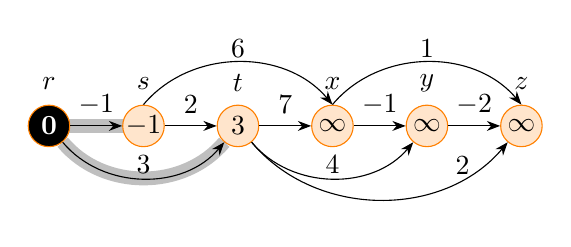
\begin{tikzpicture}[dgraph]
\def\a{1.2}
\node["$r$" {above}, bnode] (r) at (0,0) {$0$};
\node["$s$" {above}] (s) at (\a,0) {$-1$};
\node["$t$" {above}] (t) at (2*\a,0) {$3$};
\node["$x$" {above}] (x) at (3*\a,0) {$\infty$};
\node["$y$" {above}] (y) at (4*\a,0) {$\infty$};
\node["$z$" {above}] (z) at (5*\a,0) {$\infty$};
\path
    (r) edge node[tt, above] {$-1$} (s)
    (s) edge node[tt, above] {$2$} (t)
    (t) edge node[tt, above] {$7$} (x)
    (x) edge node[tt, above] {$-1$} (y)
    (y) edge node[tt, above] {$-2$} (z)
    (r) edge[bend right=50] node[tt, yshift=5pt] {$3$} (t)
    (s.north) edge[bend left=50] node[tt, yshift=5pt] {$6$} (x.north)
    (x.north) edge[bend left=50] node[tt, yshift=5pt] {$1$} (z.north)
    (t) edge[bend right=50] node[tt, yshift=5pt] {$4$} (y)
    (t) edge[bend right=50] node[tt, yshift=5pt, pos=0.8] {$2$} (z)
;
\scoped[on background layer]{
    \draw[emph] (r.center) -- (s.center);
    \draw (r) edge[-,emph,bend right=50] (t);
}
\end{tikzpicture}\hspace{2cm}\input{tikz/dag3}
\input{tikz/dag4}\hspace{2cm}\input{tikz/dag5}
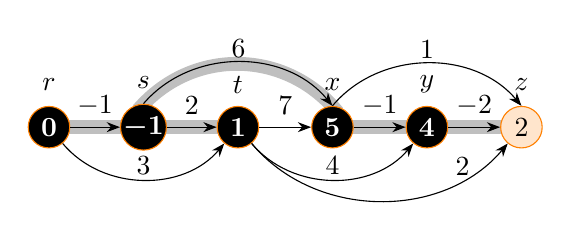
\begin{tikzpicture}[dgraph]
\def\a{1.2}
\node["$r$" {above}, bnode] (r) at (0,0) {$0$};
\node["$s$" {above}, bnode] (s) at (\a,0) {$-1$};
\node["$t$" {above}, bnode] (t) at (2*\a,0) {$1$};
\node["$x$" {above}, bnode] (x) at (3*\a,0) {$5$};
\node["$y$" {above}, bnode] (y) at (4*\a,0) {$4$};
\node["$z$" {above}] (z) at (5*\a,0) {$2$};
\path
    (r) edge node[tt, above] {$-1$} (s)
    (s) edge node[tt, above] {$2$} (t)
    (t) edge node[tt, above] {$7$} (x)
    (x) edge node[tt, above] {$-1$} (y)
    (y) edge node[tt, above] {$-2$} (z)
    (r) edge[bend right=50] node[tt, yshift=5pt] {$3$} (t)
    (s.north) edge[bend left=50] node[tt, yshift=5pt] {$6$} (x.north)
    (x.north) edge[bend left=50] node[tt, yshift=5pt] {$1$} (z.north)
    (t) edge[bend right=50] node[tt, yshift=5pt] {$4$} (y)
    (t) edge[bend right=50] node[tt, yshift=5pt, pos=0.8] {$2$} (z)
;
\scoped[on background layer]{
    \draw[emph] (r.center) -- (s.center);
    \draw[emph] (s.center) -- (t.center);
    \draw[emph] (x.center) -- (y.center);
    \draw[shorten <=-3pt, shorten >=-3pt] (s.north) edge[-,emph,bend left=50] (x.north);
    \draw[emph] (y.center) -- (z.center);
}
\end{tikzpicture}\hspace{2cm}\input{tikz/dag7}
\end{center}
\item[(b)]
$D^{(0)} = 
\begin{pmatrix}
0 & \infty & \infty & \infty & 1 & \infty \\
1 & 0 & \infty & 2 & \infty & \infty \\
\infty & 2 & 0 & \infty & \infty & -8 \\
-4 & \infty & \infty & 0 & 3 & \infty \\
\infty & 7 & \infty & \infty & 0 & \infty \\
\infty & 5 & 10 & \infty & \infty & 0 \\
\end{pmatrix}$
$D^{(1)} = 
\begin{pmatrix}
0 & \infty & \infty & \infty & 1 & \infty \\
1 & 0 & \infty & 2 & 2 & \infty \\
\infty & 2 & 0 & \infty & \infty & -8 \\
-4 & \infty & \infty & 0 & -3 & \infty \\
\infty & 7 & \infty & \infty & 0 & \infty \\
\infty & 5 & 10 & \infty & \infty & 0 \\
\end{pmatrix}$

$D^{(2)} = 
\begin{pmatrix}
0 & \infty & \infty & \infty & 1 & \infty \\
1 & 0 & \infty & 2 & 2 & \infty \\
3 & 2 & 0 & 4 & 4 & -8 \\
-4 & \infty & \infty & 0 & -3 & \infty \\
8 & 7 & \infty & 9 & 0 & \infty \\
6 & 5 & 10 & 7 & 7 & 0 \\
\end{pmatrix}$
$D^{(3)} = 
\begin{pmatrix}
0 & \infty & \infty & \infty & 1 & \infty \\
1 & 0 & \infty & 2 & 2 & \infty \\
3 & 2 & 0 & 4 & 4 & -8 \\
-4 & \infty & \infty & 0 & -3 & \infty \\
8 & 7 & \infty & 9 & 0 & \infty \\
6 & 5 & 10 & 7 & 7 & 0 \\
\end{pmatrix}$

$D^{(4)} = 
\begin{pmatrix}
0 & \infty & \infty & \infty & 1 & \infty \\
-2 & 0 & \infty & 2 & -1 & \infty \\
0 & 2 & 0 & 4 & 1 & -8 \\
-4 & \infty & \infty & 0 & -3 & \infty \\
5 & 7 & \infty & 9 & 0 & \infty \\
3 & 5 & 10 & 7 & 4 & 0 \\
\end{pmatrix}$
$D^{(5)} = 
\begin{pmatrix}
0 & 8 & \infty & 10 & 1 & \infty \\
-2 & 0 & \infty & 2 & -1 & \infty \\
0 & 2 & 0 & 4 & 1 & -8 \\
-4 & 4 & \infty & 0 & -3 & \infty \\
5 & 7 & \infty & 9 & 0 & \infty \\
3 & 5 & 10 & 7 & 4 & 0 \\
\end{pmatrix}$

$D^{(6)} = 
\begin{pmatrix}
0 & 8 & \infty & 10 & 1 & \infty \\
-2 & 0 & \infty & 2 & -1 & \infty \\
-5 & -3 & 0 & -1 & -4 & -8 \\
-4 & 4 & \infty & 0 & -3 & \infty \\
5 & 7 & \infty & 9 & 0 & \infty \\
3 & 5 & 10 & 7 & 4 & 0 \\
\end{pmatrix}$
\label{p1:b}
\item[(c)] The final shortest distance matrix is the same as $D^{(6)}$ in (b):
$\begin{pmatrix}
0 & 8 & \infty & 10 & 1 & \infty \\
-2 & 0 & \infty & 2 & -1 & \infty \\
-5 & -3 & 0 & -1 & -4 & -8 \\
-4 & 4 & \infty & 0 & -3 & \infty \\
5 & 7 & \infty & 9 & 0 & \infty \\
3 & 5 & 10 & 7 & 4 & 0 \\
\end{pmatrix}$\\
$h(a, b, c, d, e, f)=(-5,3,0,-1,-4,-8)$.\\
The graph after reweighting with $\hat{w}(u, v)=w(u, v)+h(u)-h(v)$:
\begin{center}
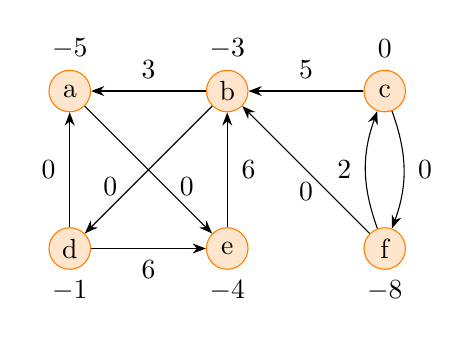
\begin{tikzpicture}[dgraph]
\def\a{2}
\node["$-5$"] (0)         at (0,\a)     {a};
\node["$-3$"] (1)         at (\a,\a)    {b};
\node["$0$"] (2)         at (\a*2,\a)   {c};
\node["$-1$" {below}] (3) at (0,0)      {d};
\node["$-4$" {below}] (4) at (\a,0)     {e};
\node["$-8$" {below}] (5) at (\a*2,0)   {f};
\path
(0) edge node[tt,above,pos=0.8] {0 } (4)
(1) edge node[tt,above] {3 } (0)
(1) edge node[tt,pos=0.8,above] {0 } (3)
(2) edge node[tt,above] {5 } (1)
(2) edge[bend left=20,right] node[tt] {0} (5)
(3) edge node[tt, left] {0 } (0)
(3) edge node[tt, below] {6 } (4)
(4) edge node[tt, right] {6 } (1)
(5) edge node[tt, below] {0 } (1)
(5) edge[bend left=20] node[tt, left] {2 } (2)
;
\end{tikzpicture}
\end{center}
\end{description}
\problem %2
The algorithms are dynamic programming on a DAG. They share the same framework:
\begin{algorithmic}[1]
    \State topologically sort the vertices of $G.V$
    \State $dp=initial(G,w)$
    \For{$u$ in topologically sorted order of $G.V$}
        \For{each $v\in G.Adj[u]$}
            \State $dp[v] = f(dp[u], dp[v], w(u, v))$
        \EndFor
    \EndFor
    \State \Return $postprocessing(dp)$
\end{algorithmic}
\newcommand{\To}[1]{\stackrel{#1}{\leadsto}}
\begin{description}
\item[(a)] Let $dp[v]$ be the number of paths in $G$ ended at $v$.
    A path to $v$ is either $?\leadsto u\to v$ (\texttt\#=$dp[u]$) or $(u, v)\in E$ (\texttt\#=1). \\
    So, $initial[i]=0$ for all vertices $i$;\\
    $dp[v] = dp[v] + dp[u] + 1$;\\
    \textbf{return} $\sum_{u\in G.V} dp[u]$.
\item[(b)] Let $dp[v]$ be the earliest starting time of job $v$. If $v$ has no incoming edge,
    then $dp[v]=0$. Otherwise, $dp[v]=\min\{dp[u]+w(u)\mid (u,v)\in E\}$. So,\\
    $initial[u]=\begin{cases}0 & \delta_{in}(u)=0\\ \infty & \delta_{in}(u)>0\end{cases}$;\\
    $dp[v]=\min\{dp[v], dp[u] + w(u)\}$;\\
    \textbf{return} $dp$.
\item[(c)] Similar to (b). $initial[u]=w(u); dp[v]=\max\{dp[v], dp[u] + w(v)\}; \textbf{return }dp$.
\end{description}
\problem %3
\textbf{This problem may be flawed, or I may not fully capture the intent of our professor.}

We want to maximize the value of:
$$R[c_j, c_{i_1}]\times R[c_{i_1},c_{i_2}]\times\cdots\times R[c_{i_k},c_j]$$
Based on the fact that the problem is modified from CLRS Problem 24-3, we will discuss the purpose of the problem.

First, can $i_x = j$? If we restrict that $i_x\neq j$, then the Traveling Salesman Problem can be reduced to this problem, which is NP-Hard. Now we assume $i_x$ can be $j$, and there is no restriction on $k$. Then, if there is an arbitrage, we have some $c_j$ that can be exchanged for an arbitrary amount of $c_j$ via the arbitrage.

Second, is $k=0$ so that the value is $R[c_j, c_j]$ a valid choice? And is {\it no exchange} a valid choice? Luckily, by proper preprocessing, the problem can be reduced to a must-exchange and $k$-can-be-$0$ variation.

\begin{table}[H]
    \centering
    \begin{tabular}{c|c|c}
      & $k$ can be $0$  & $k\ge 1$ \\\hline
      Allow no exchange & Set $R[c_j,c_j]=\max\{R[c_j,c_j],1\}$ & Not sound  \\\hline
      Must do exchanges & The standard version & Set $R[c_j,c_j]=0$
    \end{tabular}
    \caption{Preprocessing in various conditions}
    \label{tab:explain}
\end{table}
Let $D(j)$ be the maximum unit of currency one unit of $c_j$ can buy. We use the Floyd-Warshall algorithm with the recurrence formula
$$d^{(k)}(i,j)=\max\{d^{(k-1)}(i,k)\times d^{(k-1)}(k,j)\}$$
At the end of Floyd-Warshall, if $c_j$ is on an arbitrage, a directed cycle that product of weights on the path $>1$, then $d^{(n)}(j,j)>1$ and $D(j)=\infty$. If $c_j$ can reach an arbitrage and the arbitrage can reach $c_j$ through positive-weight edges, then $D(j)=\infty$. In both cases, $c_j$ and the arbitrage are in a strongly connected component. If the SCC of $c_j$ does not contain an arbitrage, then $D(j)=d^{(n)}(j,j)$.\\[1em]
\ta{MaxProduct}($R[1..n, 1..n]$)
\begin{algorithmic}[1]
\State $G=([1..n], \{(i, j)\mid R(i,j)>0\})$
\State $\ta{TarjanSCC}(G)$
\For{$k=1$ to $n$}
    \For{$i=1$ to $n$}
        \For{$j=1$ to $n$}
            \State $R[i,j]=\max\{R[i,j],R[i,k]\times R[k,j]\}$
        \EndFor
    \EndFor
\EndFor
\State Initialize $arbit[1..|SCC|]$ to $\it False$
\For{$i=1$ to $n$}
    \If{$R[i,i]>1$}
        \State $arbit[i.\it SCC]=True$
    \EndIf
\EndFor
\For{$i=1$ to $n$}
    \If{$arbit[i.\it SCC]$}
        \State $D[i]=\infty$
    \Else
        \State $D[i]=R[i,i]$
    \EndIf
\EndFor
\State Return $D$
\end{algorithmic}
The running time is $O(n^3)$.

\problem %4
Let $dp[i,u]$ be the length of the shortest path from source $v$ to vertex $u$ using exactly $i$ edges.

The base case: $dp[0,v] = 0$ (The distance to the source using 0 edges is 0). All other $dp[0,u] = \infty$.

For each step $i$ from $1$ to $k$, we compute the shortest path using exactly $i$ edges based on the values computed for $i-1$ edges.

To reach vertex $z$ with $i$ edges, we must have reached some neighbor $u$ (which has a directed edge to $z$) using $i-1$ edges, and then traversed the edge $(u, z)$. So,
$$dp[i,z] = \min\{dp[i,z], \ dp[i-1,u] + weight(u,z)\}$$
\ta{ShortestLengthKPath}$(G, weight, v, w, k)$
\begin{algorithmic}[1]
\State Initialize $pre[1..n]$ with $\infty$
\State $pre[v]=0$
\For{$i=1$ to $k$}
    \State Fill $cur[1..n]$ with $\infty$
    \For{each $(u,z)\in G.E$}
        $cur[z] = \min\{cur[z], pre[u]+weight(u, z)\}$
    \EndFor
    \State $pre = cur$
\EndFor
\State \Return $pre[w]$
\end{algorithmic}\vspace{1em}
The running time is $O(kE)$.
\problem %5
\begin{description}
\item[(a)] \textbf{Yes}. Suppose that to optimally parenthesize $A_i\cdots A_j$, we split between $A_k$ and $A_{k+1}$. Then the way we parenthesize $A_i\cdots A_k$ and $A_{k+1}\cdots A_j$ is optimal. Otherwise, we can substitute that parenthesization to produce another way to parenthesize $A_i\cdots A_j$ whose cost is higher than the optimum. Contradictory.
\item[(b)] \textbf{No}. The way we cut the rod on one side effects the number of pieces we can use on the other side. Suppose the length of the rod is $4$, and $l_1=2,l_2=1$. If we cut the rod in the middle. Then, cutting the left sub-rod into $[1, 1]$ or $[2]$ affects whether the right sub-rod can be cut into $[1, 1]$. The subproblems are not independent.
\end{description}
\problem %6
This problem is a classic variation of the Matrix Chain Multiplication problem or the Optimal Binary Search Tree problem. It can be solved using Dynamic Programming.
\paragraph{Definitions} Add parentheses to change the order of evaluation to maximize the value of the expression
    $$c_1 x_1 c_2 x_2 c_3 ... c_n x_n$$
  where $x_i$ are non-negative integers, $c_i$ are $+$ or $-$, and $c_1 = +$.
\paragraph{Optimal substructure and recursion} Any parenthesized expression can be split into two smaller sub-expressions at the last operator to be evaluated. Let $Max(i, j),\,Min(i, j)$ be the maximum/minimum value of the sub-expression ranging from $x_i$ to $x_j$. Consider the last operator $c_k$.
\begin{enumerate}
    \item $+$: $f(i, j) = f(i, k-1) + f(k, j),\,f=Max, Min$
    \item $-$: $f(i, j) = f(i, k-1) + f'(k, j),\,f=Max, Min, f'=Min, Max$
\end{enumerate}

\begin{minipage}{\textwidth}
\ta{Max-Parenthesized-Expression}$(c[1..n], x[1..n])$
\begin{algorithmic}[1]
\For{$i=1$ to $n$}
    \State $M[i,i]=m[i,j]=x[i]$
\EndFor
\For{$l=2$ to $n$}
    \For{$i=1$ to $n-l+1$}
        \State $j=i+l-1$
        \State $M[i,j]=-\infty, m[i,j]=\infty$
        \For{$k=i+1$ to $j$}
            \If{$c[k]=+$}
                \State $M[i,j] = \max\{M[i,j], M[i,k-1] + M[k,j]\}$
                \State $m[i,j] = \min\{m[i,j], m[i,k-1] + m[k,j]\}$
            \Else
                \State $M[i,j] = \max\{M[i,j], M[i,k-1] - m[k,j]\}$
                \State $m[i,j] = \min\{m[i,j], m[i,k-1] - M[k,j]\}$
            \EndIf
        \EndFor
    \EndFor
\EndFor
\State \Return $M[1,n]$
\end{algorithmic}
\end{minipage}
\vspace{1em}
The running time is $\sum_{l=2}^{n}(n-l+1)(l-1)=O(n^3)$.

\paragraph{Greedy} Yes! This problem has a greedy solution. \verb|eval|$(c)$ be all possible sign configurations reachable by parenthesizing the expression with sign array $c$.
The relation can be recursively defined in Rocq:
\begin{minted}{coq}
Inductive sign := P | N.

Definition neg (s: sign) : sign :=
  match s with
  | P => N
  | N => P
  end.

Inductive eval : list sign -> list sign -> Prop :=
| eval_nil : eval [] []
| eval_P : forall l l' r r',
    eval l l' ->
    eval r r' ->
    eval (l ++ P :: r) (l' ++ P :: r')
| eval_N : forall l l' r r' r'',
    eval l l' ->
    eval r r' ->
    map neg r' = r'' ->
    eval (l ++ N :: r) (l' ++ N :: r'').
\end{minted}

We only need to consider \verb|greedy_eval|$(c)$, defined as:
\begin{minted}{coq}
Inductive greedy_eval : list sign -> list sign -> Prop :=
| greedy_eval_refl : forall l, greedy_eval l l
| greedy_eval_flip : forall l1 l2 n,
    greedy_eval
      (l1 ++ N :: repeat P n ++ N :: l2)
      (l1 ++ N :: repeat N n ++ P :: repeat P (length l2)).
\end{minted}
This is because \verb|greedy_eval| is sound and complete (it is a subset of \verb|eval| and contains the largest one).
\begin{minted}{coq}
Theorem greedy_eval_sound :
  forall l l', greedy_eval l l' -> eval l l'.
  
Fixpoint value (l : list (sign * nat)) : Z :=
  match l with
  | [] => 0
  | (P, x) :: tl => (Z.of_nat x + value tl)%Z
  | (N, x) :: tl => (- Z.of_nat x + value tl)%Z
  end.

Definition weaker l l' := forall values,
  (value (combine l values) <= value (combine l' values))%Z.

Definition greedy_eval_complete_spec :=
  forall l l',
    eval l l' ->
    exists L,
      (weaker l' L) /\
      greedy_eval l L.
\end{minted}

\def\svgwidth{0.8\textwidth}
\begin{figure}[H]
    \center
    \import{svg}{define_dep.pdf_tex}
    \caption{The dependent graph of definitions for theorem \texttt{greedy\_eval\_complete}}
    \label{fig:define_dep}
\end{figure}

\begin{minipage}{\textwidth}
\ta{MaxParenthesis}$(c[1..n], x[1..n])$
\begin{algorithmic}[1]
\State $sum[0]=0$
\State $sumx[0]=0$
\For{$i=1$ to $n$}
\State $sum[i]=sum[i-1]+c_i\times x_i$
\State $sumx[i]=sumx[i-1]+x_i$
\EndFor
\State $ans=sum[n]$
\For{$i=1$ to $n-1$}
    \If{$c[i]=+$}
    \State \textbf{continue}
    \EndIf
    \For{$j=i+1$ to $n$}
    \If{$c[j]=-$}
        \State $ans=\max\{ans, sum[i]-(sumx[j-1]-sumx[i])+sumx[n]-sumx[j-1]\}$
        \State \textbf{break}
    \EndIf
    \EndFor
\EndFor
\State \Return $ans$
\end{algorithmic}
\end{minipage}\vspace{1em}
The greedy algorithm runs in $O(n)$.
Complete proof file is here \url{https://github.com/top-mind/alg2025_nju/blob/master/parenthesis.v}.
\end{document}